\chapter{Methodologie}
\label{hoofdstuk:methodologie}

We zullen zowel bij het vergelijken van de uiteindelijke algoritmes in hoofdstuk \ref{hoofdstuk:resultaten} als bij het vergelijken van verschillende technieken en parameterwaarden in hoofdstuk \ref{hoofdstuk:tucker} en hoofdstuk \ref{hoofdstuk:hervorming} experimenten uitvoeren om onze conclusies te staven. Om deze reden zullen we eerst alle nodige context voor deze experimenten beschrijven in dit hoofdstuk.

\section{Algemeen}
Om rekening te houden met variantie, zullen tijdsmetingen in deze tekst uitgemiddeld worden over 10 experimenten, tenzij anders vermeld. Technisch gezien zijn de resultaten van stochastische algoritmen ook niet compleet deterministisch, maar aangezien de variantie hierop vaak minimaal is zal de nood aan een grotere steekproef geval per geval behandeld worden. Daarnaast zullen tijdsmetingen ook uitgedrukt worden in CPU-tijd.

\section{Hardware}
Tenzij anders vermeld werden de tijdsmetingen in deze tekst uitgevoerd op \'e\'en core van een Intel(R) Core(TM) i7-4700HQ CPU @ 2.40GHz processor met 6GB RAM.

\section{Compressiefactor}

De compressiefactor is een belangrijke variabele die we zullen gebruiken in deze thesis. Hiermee hebben we het over de verhouding tussen de grootte van de originele, ongecomprimeerde 3D-tensor (dus bijvoorbeeld voor een $100 \times 100 \times 10$ tensor bestaande uit 16-bit integers is dit 200000 bytes) en de grootte van de gecomprimeerde versie (met als datatype voor niet-gehele getallen 32-bit floats, tenzij anders vermeld). Dit is echter een erg simpel formaat en niet altijd de beste manier om deze data op te slaan. Men moet er dus rekening mee houden dat men alleen al door de rauwe data op te slaan in een Zip-archief een compressiefactor van bijvoorbeeld 1.35 kan bekomen. Bijgevolg dient deze factor vooral relatief bekeken te worden, om verschillende compressietechnieken met elkaar te kunnen vergelijken.\\

Verder zal het geheugengebruik van metadata (onder meer afmetingen van tensoren, compressieparameters en modevolgorde) verwaarloosd worden, aangezien dit veel kleiner is dan de benodigde opslagruimte voor tensoren en matrices. Concreet betekent dit dat we alleen geheugenruimte zullen meetellen van objecten die in een zekere zin groeien met de grootte van de invoer, behalve als deze groeien met het aantal dimensies van de tensoren waarmee we werken (aangezien dit in de praktijk toch heel beperkt is).

\section{Compressiefout}

Om de fouten ge\"introduceerd door de lossy compressie te vergelijken, zullen we werken met de relatieve fout, gedefinieerd als:

\[
\text{relatieve fout} = \frac{||\text{gereconstrueerde tensor} - \text{originele tensor}||_F}{||\text{originele tensor}||_F}
\]

\section{Implementatie}

De implementatie van de besproken algoritmen gebeurde in Python, waarbij het zware rekenwerk werd uitgevoerd via library calls, voornamelijk aan de hand van NumPy, SciPy en zlib. Hierbij zijn ook alternatieve strategie\"en getest (zoals het al dan niet minimaliseren van transposities, het gebruik van \texttt{numpy.einsum}, ...), waarbij telkens de meest performante werd gekozen. Deze keuzes zullen weinig behandeld worden in deze tekst vanwege de sterke afhankelijkheid van de gekozen programmeertaal. Desalniettemin kan het dat er nog steeds merkbare ineffici\"enties in de implementatie zijn.\\

Om enkele verschillende encoderingen effici\"ent te kunnen uitvoeren, hebben we niet alleen de Python-module \texttt{bitarray} \cite{ref:bitarray} gebruikt, maar deze ook uitgebreid met enkele methodes (zie sectie \ref{sec:encodering} voor meer informatie). Deze code werd, zoals de rest van de module, in C geschreven voor performantie.\\

Zoals eerder vermeld, zullen de belangrijkste stukken broncode toegevoegd worden als bijlage. Om de lengte van deze tekst te beperken, zal niet de volledige code aanwezig zijn in deze bijlagen, maar deze is beschikbaar via de \textit{repository}: \url{https://github.com/Wout12345/hyperspectral-image-compression-co}

\section{Datasets}

Om een idee te krijgen van de effici\"entie van de verschillende compressietechnieken, moet men gebruik maken van echte hyperspectrale afbeeldingen. Hieronder volgen enkele voorbeelden met hun bijbehorende eigenschappen. De afbeeldingen zijn slechts een 2D-voorstelling van de hyperspectrale data, verkregen door alle frequentiekanalen bij elkaar op te tellen en deze sommen voor te stellen met grijswaarden. Dit zijn ook telkens voorstellingen van de finale datasets waarmee we werken, zonder eventuele verwijderde spatiale en spectrale banden.\\

Bij de voorverwerking zullen we vaak bepaalde spectrale banden weglaten indien blijkt dat deze artefacten bevatten (onder meer banden met waarde 0, banden met veel te hoge, willekeurig verdeelde intensiteiten en naburige banden). Op spatiaal vlak zullen we soms de afmetingen naar beneden afronden tot het dichtsbijzijnde kwadraat; hierdoor kan men deze assen eventueel later nog makkelijk reshapen. Verder is het ook in sommige gevallen nodig om een geroteerde in plaats van as-gealigneerde rechthoek te selecteren. Hierbij vallen de roosterpunten in het nieuwe assenstelsel niet exact op oude roosterpunten en zal de nieuwe dataset gereconstrueerd worden door bilineair te interpoleren \cite{ref:bilinear_interpolation} over de twee spatiale assen.\\

Omdat de geproduceerde bestanden te groot zijn om in bijlage toe te voegen en deze voorverwerking niet triviaal is om formeel te beschrijven, hebben we de code van de voorverwerker toegevoegd in bijlage \ref{app:voorverwerker}. Men kan deze combineren met de originele data van de corresponderende bronnen om dezelfde datasets te reproduceren.

\subsection{Indian Pines}

\begin{figure}[H]
  \centering
  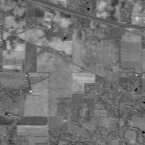
\includegraphics[scale=1]{images/indian_pines_sum.png}
  \caption{Indian Pines, VS. Bron: AVIRIS \cite{ref:ehu_aviris_indian_pines}}
  \label{fig:indian_pines_sum}
\end{figure}

\textbf{Spatiale dimensies:} $145 \times 145$\\
\textbf{Spectrale dimensie:} 220\\
\textbf{Voorverwerking:} Geen.

\newpage
\subsection{Cuprite}

\begin{figure}[H]
  \centering
  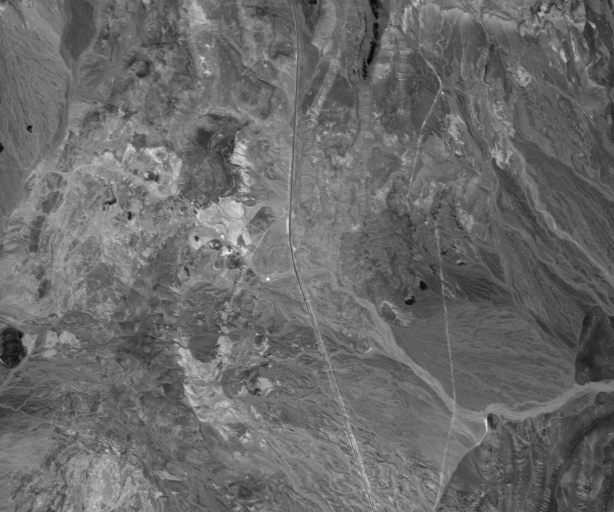
\includegraphics[scale=0.5]{images/cuprite_sum.png}
  \caption{Cuprite, VS. Bron: AVIRIS \cite{ref:ehu_aviris_cuprite}}
  \label{fig:cuprite_sum}
\end{figure}

\textbf{Spatiale dimensies:} $512 \times 614$\\
\textbf{Spectrale dimensie:} 190\\
\textbf{Voorverwerking:} De originele spectrale dimensie was 224, maar banden 0-3, 106-113, 152-168 en 219-223 werden verwijderd.

\newpage
\subsection{Pavia Centre}

\begin{figure}[H]
  \centering
  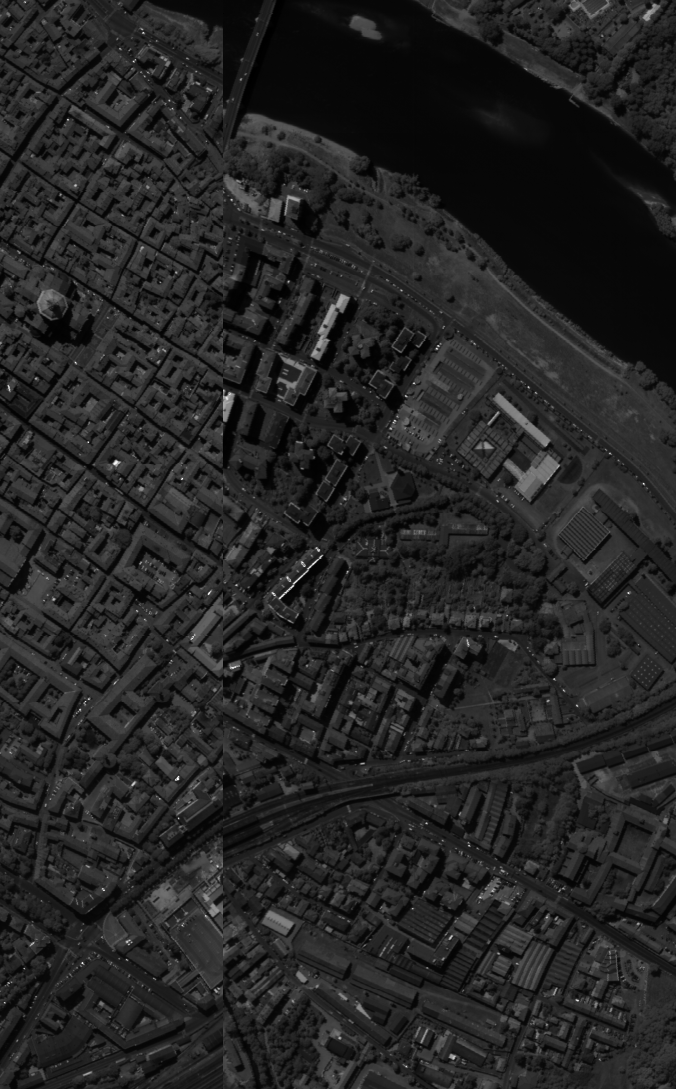
\includegraphics[scale=0.4]{images/pavia_sum.png}
  \caption{Pavia Centre, Itali\"e. Bron: ROSIS \cite{ref:ehu_rosis}}
  \label{fig:pavia_sum}
\end{figure}

\textbf{Spatiale dimensies:} $1089 \times 676$\\
\textbf{Spectrale dimensie:} 102\\
\textbf{Voorverwerking:} De download van de EHU \cite{ref:ehu_rosis} heeft al een reeks spatiale banden zonder informatie weggelaten en heeft spatiale dimensies $1096 \times 715$. Hiervan selecteerden we de pixels met de laagste indices. De weggelaten rijen en kolommen zouden zich dus onder en rechts van de afbeelding hierboven bevinden.

\newpage
\subsection{Mauna Kea}

\begin{figure}[H]
\centering
\begin{subfigure}{.5\textwidth}
  \centering
  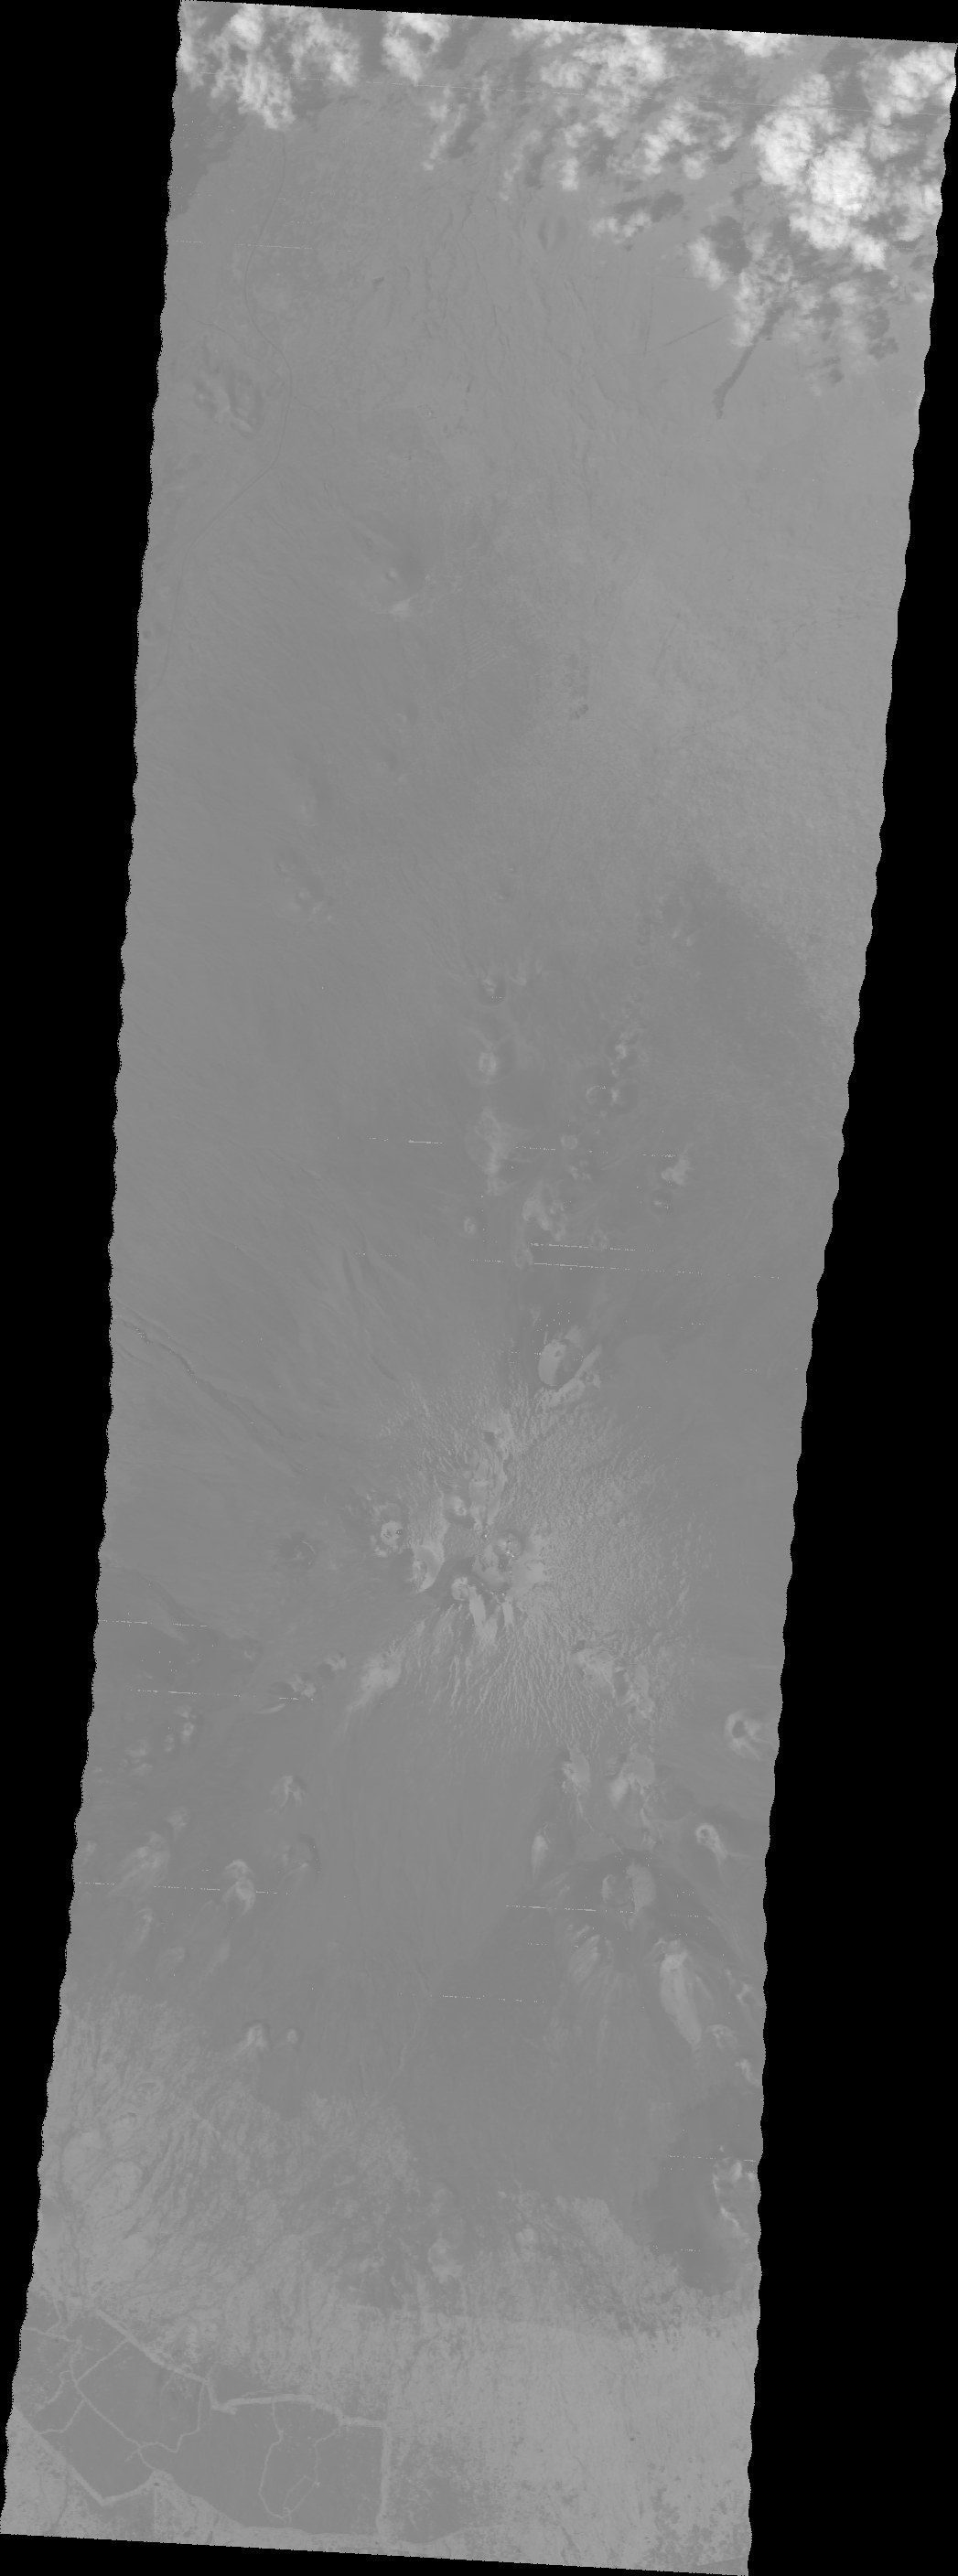
\includegraphics[scale=0.14]{images/mauna_kea_raw_sum.png}
  \caption{Origineel}
\end{subfigure}%
\begin{subfigure}{.5\textwidth}
  \centering
  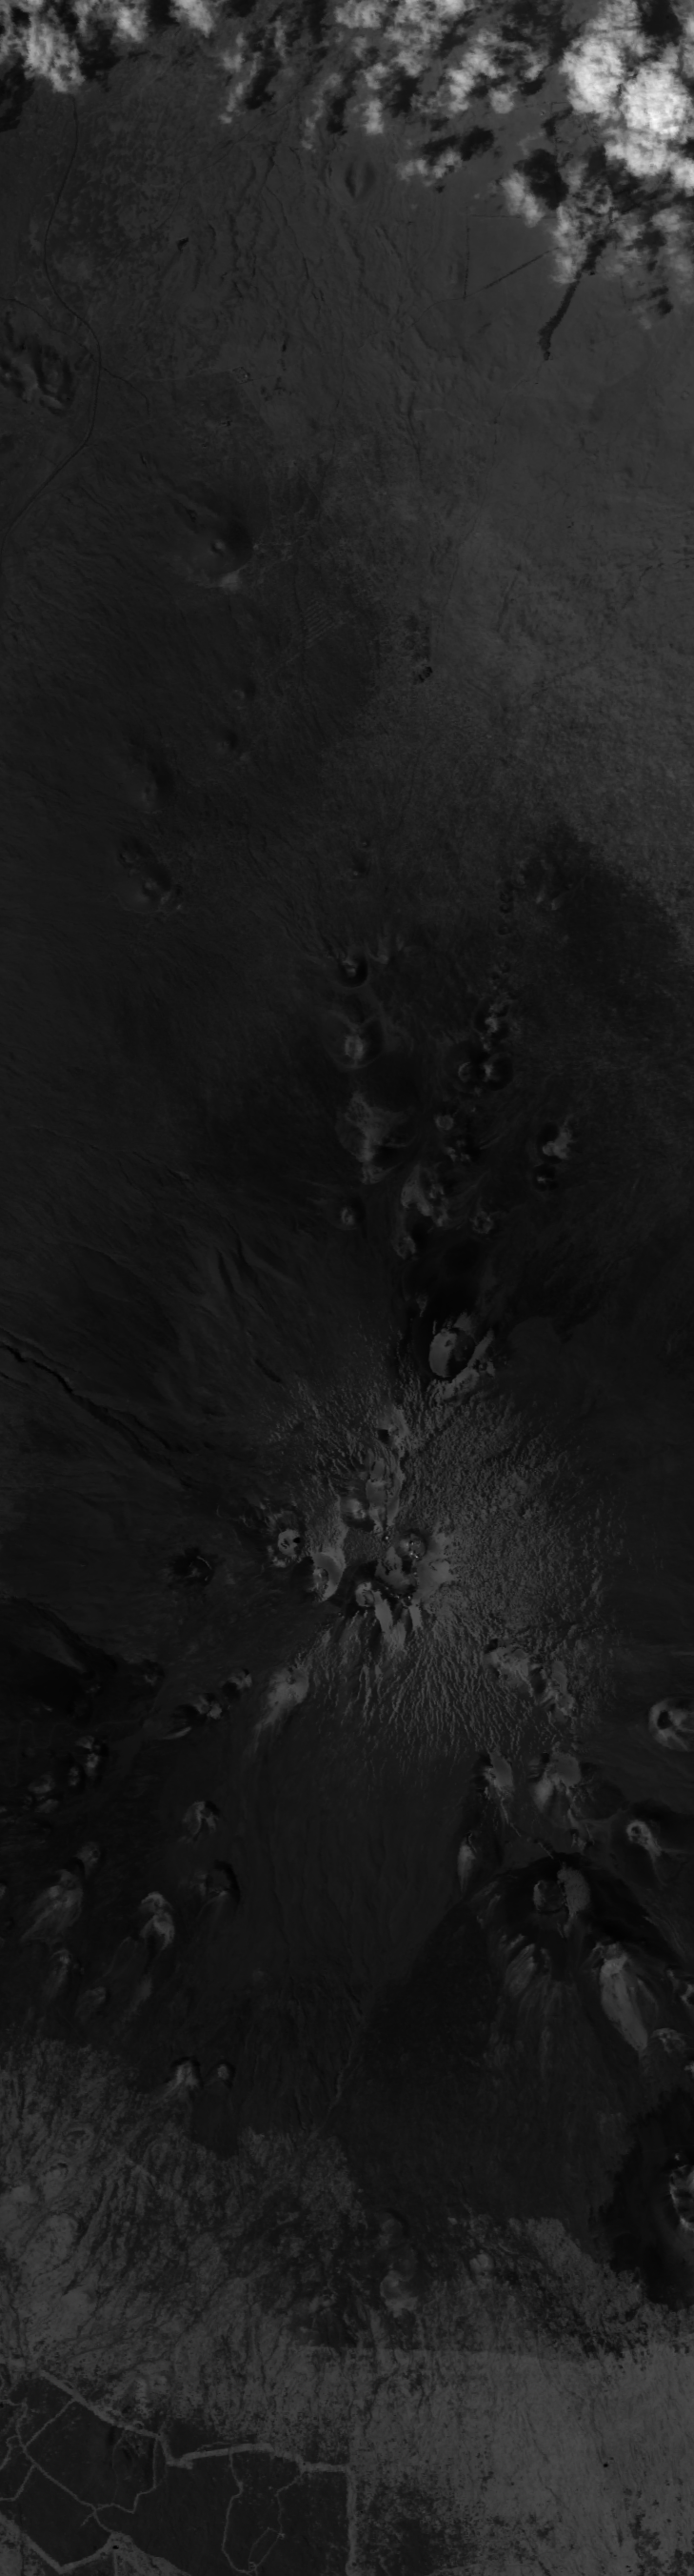
\includegraphics[scale=0.14]{images/mauna_kea_sum.png}
  \caption{Na voorverwerking}
\end{subfigure}
\caption{Mauna Kea, VS. Bron: AVIRIS \cite{ref:aviris}}
\label{fig:mauna_kea}
\end{figure}

\textbf{Spatiale dimensies:} $2704 \times 729$\\
\textbf{Spectrale dimensie:} 199\\
\textbf{Voorverwerking:} Op spatiaal vlak werd een rechthoek geselecteerd, beginnend in (40, 240) en 4.07 graden wijzerzin gedraaid ten opzichte van het originele assenstelsel. Op spectraal vlak werden van de 224 originele banden de banden 0-1, 103, 107-113 en 153-167 verwijderd. Hierna werden alle waarden verschoven en geschaald zodat het bereik ervan exact overeenkomt met dat van unsigned 16-bit integers, het data type dat ook voor de andere datasets gebruikt werd.